\documentclass[a4paper,chapter,microtype,fleqn,oneside]{oblivoir}
\usepackage[hangul]{kotex}
\usepackage[inner=1.1in,outer=1.1in]{geometry}
\usepackage{graphicx}
\usepackage{wrapfig}
\usepackage[style=authoryear-comp,sortcites=false,uniquename=false,maxnames=4,minbibnames=99,maxbibnames=99,dashed=false,backref=true,backrefstyle=none]{biblatex}
\usepackage{tcolorbox}
\usepackage{csquotes}
\usepackage{amsmath}
\usepackage{amsthm}
\usepackage{amssymb}
\usepackage{etoolbox}
\usepackage{caption}
\usepackage{multido}
\usepackage{enumitem}


\definecolor{box-background}{RGB}{242,242,242}
\definecolor{box-frame}{RGB}{64,64,64}
\newenvironment{rbox}[1]{\begin{tcolorbox}[colback=box-background,colframe=box-frame,title=\textbf{#1}]}{\end{tcolorbox}}

\newtheoremstyle{rlai}%
  {\topsep}{\topsep}%
  {\normalfont}{0pt}%
  {\bfseries}{ }%
  {5pt plus 1pt minus 1pt}%
  {{\bfseries\thmname{#1} \thmnumber{#2}:} \thmnote{\itshape#3}}
\theoremstyle{rlai}
\newtheorem{exercise}{연습 문제}[chapter]
\AtEndEnvironment{exercise}{\null\hfill\ensuremath{\square}}
\newtheorem{example}{사례}[chapter]
\AtEndEnvironment{example}{\null\hfill\ensuremath{\blacksquare}}

\oblivoirchapterstyle{default}

\DeclareMathOperator*{\argmax}{arg\,max}




\renewcommand*{\nameyeardelim}{\addcomma\space}
\DeclareNameAlias{author}{last-first}

\addbibresource{rlai.bib}

\DeclareBibliographyAlias{customa}{misc}
\DeclareBibliographyAlias{customb}{misc}

\renewcommand*{\finalnamedelim}{%
  \ifcitation{
    \ifnumgreater{\value{liststop}}{2}{\finalandcomma}{}%
    \addspace\bibstring{and}\space%
  }{
    \ifentrytype{customa}{%
      \ifnumgreater{\value{liststop}}{2}{\finalandcomma}{}%
      \addspace\bibstring{and}\space%
    }{%
      \finalandcomma\addspace%
    }%
  }%
}
\renewcommand*{\bibfont}{\footnotesize}



\begin{document}

\tableofcontents


% page 1

\chapter{소개}

학습에 대해 생각할 때 아마도 가장 먼저 떠오르는 생각은 우리가 환경과
상호작용하며 배운다는 것이다. 갓난아이가 팔을 흔들며 둘러볼 때 어떻게 하라고
알려주는 사람이 없지만, 유아는 감각운동적으로 환경과 직접 연결돼있다. 감각운동을
연습하면 인과 관계와 행동의 결과 그리고 목적을 달성하기 위한 행동 순서에 대한
풍부한 정보가 쌓인다. 살면서 이런 상호작용을 통해 환경과 우리 자신에 대한
대부분의 지식을 얻는다. 운전이나 대화하는 방법을 배울 때 우리는 환경이 우리
행동에 어떻게 반응하는지 민감하게 인식하며 앞으로 일어날 일에 영향을 주려고
행동한다. 상호작용을 통한 학습이 거의 모든 학습과 지능 이론의 근간이 된다.

이 책은 상호작용을 통한 학습을 \emph{계산적으로} 접근하는 방법을 탐구한다.
사람과 동물이 어떻게 학습하는지를 직접 이론화하기보다는 이상적인 학습 환경을
살펴보고 다양한 학습 기법의 효율성을 평가한다. 즉, 우리는 인공지능 연구자나
공학자의 관점으로 본다. 과학적 혹은 경제적으로 가치가 있는 학습 문제를
효율적으로 푸는 기계를 어떻게 설계할지 탐구한다. 각각의 설계를 수학적으로
분석하거나 컴퓨터로 실행하여 검토해본다.
\emph{강화학습(reinforcement learning)}이라는 우리의 접근 방식은 다른 기계학습
보다 상호작용을 통한 훨씬 더 목표 지향적인 학습에 집중한다.

\section{강화학습}

강화학습 문제는 숫자로 된 보상 신호를
최대로 늘리기 위해 무엇을 할지 (어떻게 상황을 행동으로 연결할지) 배우는 것이다.
학습자는
무슨 행동을 할지 지시받지 않는다. 대신 직접 시도해가며 어떤 행동이 가장 많은
보상을 주는지 발견해야 한다. 흥미롭고 도전적인 대부분의 사례에서 행동은 당장의
보상뿐 아니라 다음 상황에 영향을 미쳐서 이후 모든 보상을 좌우한다.
시행착오(trial-and-error) 탐색과 지연된 보상이 강화학습의 가장 중요한 두가지
특징이다.

기계학습(machine learning)과 등산(mountaineering)과 같이 이름이 ``ing''로 끝나는
강화학습은 해결할 문제이자 동시에 이런 문제에 효과적인 해결책이며 이런 문제와
해결 방법을 연구하는 분야이기도 한다. 이 세 가지에 이름 한 개를 사용하면
편하지만, 개념상 셋을 반드시 구분해야 한다. 특히 문제와 해결책을 구분하는 것은
강화학습에서 매우 중요하다. 구분하지 못하면 이런저런 혼란이 시작한다.

동적 시스템 이론, 특히 마르코프 결정 프로세스(Markov decision process, MDP)라고
불완전하게 알려진 최적 제어 분야의 개념을 사용하여 강화학습 문제를 기술한다. 이
표현에 대한 자세한 내용은 \ref{ch:finite-markov-decision-processes}장에 가서야
다루지만, 이
기본 발상은 목표를 달성하기 위해 환경과 장시간 상호작용하는 학습 에이전트의 실제
문제에서 가장 중요한 측면이다. 학습 에이전트는 어느 정도 자신의 환경 상태를
파악할 수 있고, 상태에 영향을 주는 행동을 취해야 한다. 마르코프 결정 프로세스는
단지 감각과
행동 그리고 목표라는 세 가지 측면을 지나치게 단순화하지 않는 선에서 가장 간단히
표현하려고 한다. 이런 문제를 푸는데 적합한 기법이라면 무엇이든지 강화학습
기법이라고 한다.

% page 2

강화학습은 현재 가장 활발하게 연구되는 기계학습 분야인
\emph{지도학습(supervised learning)}과 다르다. 강화학습은 지식을 가진 외부
감독자가 라벨을 붙인 예제로 구성된 훈련 세트를 가지고 학습한다. 예제는 상황
설명과 함께 (보통은 상황이 어떤 분류에 속하는지 파악하기 위해) 그 상황에서
시스템의 올바른 행동(라벨)을 지시한다. 이런 학습의 목표는 반응을 추론하고
일반화하여 훈련 세트에 없는 상황에서도 시스템이 올바로 동작하게 만드는 것이다.
중요한 학습 분야이지만, 이것만으로는 상호작용으로 배우는데 충분하지 않다. 보통은
상호작용 문제에서 올바르고 에이전트가 만나는 모든 상황을 대표하는 바람직한
행동을 알기 어렵다. 학습이 절실한 미지의 영역에서 에이전트는 자신의 경험을 통해
배울 수 있어야 한다.

또한 강화학습은 기계학습 연구자들이 \emph{비지도학습(unsupervised
learning)}이라고 부르는 것과도 다르다. 대개
비지도학습은 라벨이 없는 자료 묶음에 숨겨진 구조를 발견하려 한다. 기계학습
분야를 지도학습과 비지도학습, 두 개만으로 나눌 수 있는 것처럼 보이지만 그렇지
않다. 올바른 행동 예제가 없어도 되기 때문에 강화학습을 비지도학습의 일종으로
보고 싶을지도 모른다. 그러나 강화학습은 숨은 구조를 찾기보다는 보상 신호를
최대로 늘리려고 노력한다. 에이전트의 경험에 숨겨진 구조를 발견하는 것도
강화학습에 도움이 되지만, 그것만으로는 보상 신호를 최대화하는 강화학습
문제를 해결할 수 없다. 그러므로 우리는 지도학습과 비지도학습 등과 더불어
강화학습을 기계학습의 세 번째 분야로 본다.

다른 종류의 학습과 달리 강화학습에서 두드러지는 어려움 중 하나는 탐색과 활용
사이의 균형이다. 많은 보상을 얻으려면, 강화학습 에이전트는 과거에 시도하여
효율적으로 보상을 준다고 알려진 행동을 선호해야 한다. 그러나 효율적으로 보상을
주는 행동을 찾으려면 과거에 선택하지 않은 행동을 시도해보아야 한다. 에이전트는
보상을 받으려면 이미 경험한 것을 \emph{활용해야(exploit)} 하지만, 또한 미래에
더 나은 선택을 하기 위해 \emph{탐색해야(explore)} 한다. 작업에 성공하려면 집중과
탐색 중 하나만 전적으로 추구하면 안 되는 점이 모순이다. 에이전트는 다양한 행동을
시도하면서 \emph{동시에} 최고로 보이는 행동을 점진적으로 선호해야 한다. 통계적
작업이라면, 에이전트는 보상의 기댓값을 신뢰할 수 있게 예측하기 위해 여러 번
시도해야 한다. 탐색-활용 모순은 수학자들이 수십 년 동안 열심히
연구했지만 아직 풀리지 않았다. 일단 탐색과 활용의 균형 문제는
최소한 순수한 형태의 지도학습과 비지도학습에는 없다고 말할 수 있다.

강화학습의 다른 특징은 불확실한 환경과 상호작용하는 목적 지향적 에이전트의 문제
\emph{전체를} 분명히 고려하는 점이다. 큰 그림에 어떻게 부합하는지 말하지 않은 채
문제의 부분들을 고려하는 여러 접근 방식과 다르다. 예를 들어, 지도학습과 연관된
상당수의 기계학습 연구는 결국 그 능력을 어떻게 유용하게 사용할지 말하지 않는다.
범용 목표를 향한 계획 이론을 개발하는 다른 연구자들은 실시간 의사결정시 계획의
역할이나 계획에 필요한 예측 모델을 어떻게 만들지 고려하지 않는다. 이런 접근
방법도 여러 유용한 결과를 달성했지만, 문제 일부분만 격리하여 고려한 점이 큰
한계이다.

% page 3

반대로 강화학습은 완전하고 상호작용하는 목적 지향 에이전트에서 시작한다. 모든
강화학습 에이전트는 명확한 목표를 가지고, 주변환경을 인지하고, 환경에 영향을
주는 행동을 선택할 수 있다. 게다가 강화학습은 처음부터 항상 매우 불확실한
주변환경에도 불구하고 에어전트는 동작해야 한다고 가정한다. 강화학습에 계획이
들어가면, 계획과 실시간 행동 선택 사이의 상호 작용과 어떻게 환경 모델을 얻고
향상할지 다루어야 한다. 강화학습에 지도학습이 들어간다면, 어떤 능력이 결정적인지
판단해야 할 이유 때문이다. 학습 연구를 진행하기 위해 중요한 문제를 부분으로
나누어 연구해야 했다. 그러나 아직 완전한 에이전트의 세부 요건을 파악할 수
없지만, 부분 문제는 완전하고 상호작용하는 목적 지향 에이전트에서 명확할 역할이
있어야 한다.

완전하고 상호작용하는 목적 지향 에이전트란 완전한 유기체나 로봇 같은 것을
뜻하지 않는다. 예를 들면, 완전하고 상호작용하는 목적 지향 에이전트는 동작하는 더
큰 시스템의 구성요소일 수도 있다. 이 경우 에이전트는 더 큰 나머지 시스템과 직접
상호작용하며 더 큰 시스템의 환경과 간접적으로 상호작용한다. 앞으로 로봇의 배터리
충전 수준을 살피고 로봇의 제어 아키텍처에 명령을 보내는 에이전트를 간단한 예로
들 것이다. 이 에이전트의 환경은 로봇의 환경과 로봇의 나머지 부분이다. 강화학습
프레임워크의 일반성을 평가하려면 가장 뻔한 에이전트와 환경 너머를 보아야 한다.

현대 강화학습의 가장 흥미로운 점 중 하나는 다른 공학과 과학 분야와 상당히 교류한
결실이다. 강화학습은 십여 년간 인공지능과 기계학습이 통계학과 최적화 그리고 다른
수학 분야와 넓게 통합하는 추세 한가운데에 있다. 예를 들어, 파라미터
근사기(parameterized approximator)를 가지고 학습하는 일부 강화학습 기법은 운용
과학(operations research)과 제어 이론의 고전적인 ``차원의 저주''를 다룬다. 또
강화학습은 심리학과 신경과학과 밀접하게 교류하며 서로에게 커다란 기여를 했다.
기계학습 분야 중에 강화학습은 인간과 다른 동물의 학습과 가장 가깝고, 강화학습의
여러 핵심 알고리즘은 원래 생물학적 학습 시스템에서 유래했다. 그리고 강화학습은
반대로 실험 결과에 더 부합하는 동물 학습의 심리적 모델과 뇌의 보상 시스템 일부에
대한 유력한 모델을 기여했다. 이 책은 공학과 인공지능에 관련된 강화학습
아이디어와 함께 \ref{ch:psychology}장과 \ref{ch:neuroscience}장에서 심리학과
신경과학과 연관성을 다룬다.

마지막으로 강화학습은 단순한 일반 이론을 향한 인공지능의 큰 추세의 일부이기도
하다. 1960년대 말 이후 많은 인공지능 연구자들은 일반 이론이란 없으며 지능은 대신
특수한 목적을 가지는 재주와 절차와 휴리스틱이 엄청나게 모인 결과라고 짐작했다.
수백만 혹은 수십억 개의 충분한 사실을 기계에 넣으면 지능이 생길 것이라는 말도
종종 있었다. 검색과 학습 같은 일반 이론에 바탕을 둔 방법은 ``약한 방법(weak
methods)''으로 분류하고, 특정 지식에 근거한 방법은 ``강한 방법(strong
methods)''이라고 불렸다. 이런 시각은 여전히 흔하지만, 지배적이지 않다. 우리가
보기에 그런 시각은 시기상조다. 일반 이론이 없다고 결론짓기에는 연구가 너무
부족했다. 현대 인공지능은 방대한 도메인 지식을 반영하려는 노력과 더불어 학습과
검색 그리고 의사결정의 일반 이론을 찾는 연구를 많이 한다. 시계추가 얼마나
돌아왔는지 확실하지 않지만, 강화학습 연구는 단순하고 적은 수의 인공지능 일반
이론을 추구한다.

% page 4

\section{사례}

강화학습의 발전을 이끈 일부 사례와 가능한 적용사례를 보면 강화학습을 이해하기
좋다.

\begin{itemize}
\item 체스 고수가 말을 움직인다. 상대방의 수와 그 다음 수를 예상한 계획과
      특정 위치와 움직임이 좋은지 순간적인 직관을 통해 어떤 말을 움직일지
      선택한다.
\item 적응 제어기는 석유 정제소 동작 파라미터를 실시간으로 조절한다. 제어기는
      기술자가 처음에 짐작한 값을 무조건 따르지 않고 지정한 한계 비용을 토대로
      생산량/비용/품질 사이의 균형을 최적화한다.
\item 새끼 가젤은 태어나고 몇 분간 일어서려고 애쓴다. 반 시간이 지나면 시간당
      30킬로미터 속력으로 달린다.
\item 이동 로봇은 쓰레기를 주으려고 새로운 방에 들어갈지 아니면 배터리 충전소로
      되돌아기 시작해야 할지 결정한다. 현재 배터리 충전 상태와 과거에 얼마나
      빠르고 손쉽게 충전소를 찾았는지를 가지고 결정을 내린다.
\item 필이 아침 식사를 준비한다. 찬장으로 걸어가기, 찬장 열기, 시리얼 상자
      선택하기, 상자로 팔을 뻗어서 상자를 잡고 가져오기. 이렇게 유심히 살펴보면
      일상적인 활동조차도 조건부 행동과 서로 맞물린 목표들 사이의 관계들이
      복잡하게 엮여있다. 그릇과 숟가락 그리고 우유병을 잡기 위해서도 일련의
      복잡하고 조화된 상호작용 동작이 필요하다. 단계별로 정보를 습득하고 손과
      운동을 안내하기 위해 눈을 움직여야 한다. 어떻게 물건을 옮기고 무엇을 먼저
      식탁으로 가져오면 좋을지를 끊임없이 빠르게 판단한다. 숟가락 잡기와
      냉장고로 이동하기 같은 목표가 매 단계를 안내하고, 이 목표들은 숟가락으로
      이미 준비한 시리얼을 먹어서 궁극에는 영양 섭취 같은 다른 목표에 기여한다.
      인지하든 모르든 관계없이 필은 자신의 몸 상태 정보를 가지고 필요한 영양분과
      배고픈 정도 그리고 선호하는 음식을 파악한다.
\end{itemize}

이 사례들은 너무 기본적이어서 간과하기 쉬운 공통된 특징이 있다. 모두 능동적인
행동 결정 에이전트와 환경 사이의 \emph{상호작용이} 있다. 환경의
\emph{불확실성에도} 불구하고 에이전트는 \emph{목표를} 달성할 방법을 찾는다.
에이전트의 행동은, 예를 들어, 다음 체스 말 위치, 정제소 비축량, 로봇의 다음
위치와 미래 배터리 충전 수준 등, 환경의 미래 상태에 영향을 주고, 그것이 다시
에이전트의 미래 선택지와 기회를 바꿀 수 있다. 올바른 선택을 하려면 행동의
간접적이고 지연된 결과를 고려해야 하고, 그래서 전망이나 계획이 필요할지 모른다.

또한, 이런 사례에서 행동의 영향을 완전히 예상할 수 없다. 그래서 에이전트는
환경을 자주 감시하고 적절하게 반응해야 한다. 예를 들어, 필은 우유를 시리얼
그릇에 부을 때 넘치지 않게 지켜봐야 한다. 모든 사례에서 에이전트는 직접 감각한
것을 가지고 목표까지 얼마나 진행했는지 판단할 수 있는 점에서 목표가 명시적이다.
체스 선수는 자신의 승패를 알고, 정제소 제어기는 석유 생산량을 알고, 이동 로봇은
언제 배터리가 바닥날지 알고, 필은 자신이 아침 식사를 즐기는지 안다.

모든 사례에서 에이전트는 경험을 통해 시간이 지나면서 나아진다. 체스 선수는
자리를 보는 통찰을 갈고닦아 결국 경기를 향상한다. 새끼 가젤은 달리기 효율을
향상한다. 필은 자연스럽게 아침 식사를 준비하는 방법을 배운다. 에이전트가 작업을
시작할 때 가진 (과거 비슷한 작업 경험 혹은 설계나 진화로 알게 된) 지식이 학습에
도움을 주지만, 작업 특성에 맞추어 행동을 조정하기 위해 환경과 상호작용은 꼭
필요하다.

% page 5

\section{강화학습의 요소}

에이전트와 환경 이외에 강화학습 시스템의 주된 요소는 \emph{정책(policy)},
\emph{보상 신호(reward signal)}, \emph{가치함수(value function)} 그리고 선택적인
환경 \emph{모델(model)}, 이렇게  네가지다.

\emph{정책(policy)}은 어떤 시점에서 학습 에이전트의 행동 방식을 정의한다. 간단히
말해서 정책은 인지된 환경 상태를 그 상태에서 취할 행동으로 대응한다. 심리학에서
일련의 자극-반응(stimulus-response) 규칙 혹은
연상(association)에 해당한다. 정책이 간단한 함수 혹은 참조표인 경우도 있고, 검색
절차같이 엄청난 계산이 필요한 정책도 있다. 정책만으로 행동을 결정하기 충분한
점에서 정책은 강화학습 에이전트의 핵심이다. 일반적으로 확률적인 정책도 가능하다.

\emph{보상 신호(reward signal)}는 강화학습 문제의 목표를 정의한다. 매시간
단계마다 환경은 \emph{보상}이라는 숫자 하나를 강화학습 에이전트에게 보낸다.
장기적인 보상 총합을 최대화하는 것이 에이전트의 유일한 목표다. 그래서 보상
신호는 에이전트에게 무엇이 좋고 무엇이 나쁜지 정의한다. 보상을 생물학적
시스템에서 즐거움이나 고통을 경험하는 것으로 생각할 수 있다. 보상은 즉시
발생하고, 에이전트가 마주한 문제를 정의하는 특징이다.
보상 신호는 보상을 변경하는 기본
근거이다. 정책으로 선택한 행동이 낮은 보상을 낸다면, 미래에 같은 상황에서 다른
상태를 선택하도록 정책을 변경할 수 있다. 일반적으로 보상 신호는 환경 상태와
선택한 행동의 확률함수이다.

보상 신호가 당장에 무엇이 좋은지 알려준다면, \emph{가치함수(value function)}는
장기적으로 무엇이 좋은지 알려준다. 쉽게 말해서 상태의 \emph{가치}는 에이전트가
그 상태부터 시작하여 앞으로 누적해서 받길 기대하는 보상의 총합이다. 보상이 환경
상태에 내재한 즉각적인 바람직함이라면, 가치는 따라갈 가능성이 높은 상태와 그
상태들의 보상들을 고려한 \emph{장기적인} 바람직함이다. 예를 들어, 당장 보상은
적지만, 그다음 상태들의 보상이 커서 가치가 높은 상태가 있을 수 있고, 반대도
가능하다. 사람에 비유하면 보상은 (높다면) 기쁨이나 (낮다면) 고통과 비슷하다면,
가치는 어떤 환경 상태에서 우리가 얼마나 즐겁고 불쾌한지를 더 원시안적으로 가늠한
것이다. 이제 가치 함수 개념에 익숙하길 바란다.

어떤 의미에서 보상은 기본적이고, 보상을 예측하는 가치는 부수적이다. 보상 없이는
가치란 있을 수 없으며 가치를 예측하는 유일한 이유는 더 많은 보상을 받기
위해서다. 그럼에도 불구하고 우리가 결정을 내리고 결정을 평가할 때 가치를 주로
고려한다. 우리는 가장 높은 보상이 아니라 가장 높은 가치를 주는 상태로 가는
행동을 추구한다. 이런 행동이 장기적으로 가장 큰 보상을 주기 때문이다. 불행하게도
보상을 측정하는 것보다 가치를 측정하기가 훨씬 어렵다. 보상은 기본적으로 환경이
직접 주지만, 가치는 짐작해야 하고 에이전트가 일생 동안 관찰한 내용을 가지고 계속
다시 가치를 추정해야 한다. 사실 효율적으로 가치를 예측하는 방법 우리가 고려할
거의 모든 강화학습 알고리즘에서 가장 중요한 요소이다. 분명히 가치 예측은 지난
수십 년 동안 강화학습 연구에서 가장 중요한 역할을 차지했다.

마지막 네 번째 강화학습 시스템 요소는 환경 \emph{모델(model)}이다. 모델은 환경의
행동을 흉내내고, 일반적으로 환경이 어떻게 동작할지 추론할 수 있게 해준다. 예를
들어, 상태와 행동이 주어지면, 모델은 다음 상태와 다음 보상을 예측할 수 있다.
\emph{계획(planning)}에도 모델을 사용한다. 계획은 실제 경험하지 않고 가능한 미래
상황을 고려하여 일련의 행동을 결정하는 방법을 말한다. 모델과 계획을 사용하여
강화학습 문제를 푸는 기법을 \emph{모델 기반(model-based)} 기법이라고 하고,
계획의 거의 \emph{반대인} 시행착오를 통해 학습하는 단순한
\emph{비모델(model-free)} 기법도 있다.
\ref{ch:planning-and-learning-with-tabular-methods}장에서 우리는 시행 착오학습과
함께 환경 모델을 학습하고 모델을 사용하여 계획하는 강화학습 시스템을 살펴볼
것이다. 현대 강화학습은 저수준의 시행착오 학습부터 고수준의 신중한 계획까지 모두
망라한다.

% page 6

\section{한계와 범위}

이제 강화학습이 상태 개념을 매우 의존함이 분명해졌다. 상태는 정책과 가치함수의
입력이며 모델의 입력이자 출력이다. 상태를 특정 시점에서 ``환경이 어떤지'' 감지할
수 있도록 에이전트에게 전달한 신호로 생각해도 된다.
\ref{ch:finite-markov-decision-processes}장에서 설명할 마르코프 결정 프로세스
구조는 여기서 말한 상태를 정식으로 정의한다. 그러나 더 일반적인, 자신의 환경에
대해 에이전트에게 알려진 정보라는, 상태의 비공식 정의를 따르길 권한다. 사실상
우리는 에이전트 환경의 명목상 일부인 전처리 시스템이 상태 신호를 만든다고
가정한다. 이 책은 환경 신호 생성과 변경 및 학습에 대해 다루지 않는다. 상태
표현이 덜 중요해서가 아니라 의사결정 문제에 완전히 집중하기 위해서이다. 즉,
우리의 주된 관심은 상태 신호 설계가 아니라 주어진 어떤 상태 신호의 함수로 어떤
행동을 취할지 결정하는 문제이다. (마지막 장
\ref{sec:observations-and-state}절에서 상태 설계와 생성을 짧게 다룬다.)

이 책에서 다루는 대부분의 강화학습 기법은 가치함수 예측과 관련이 있지만,
강화학습 문제를 풀기 위해 반드시 가치함수를 추정할 필요는 없다. 예를 들어,
그동안 가치함수 없이도 유전 알고리즘, 유전 프로그래밍, 시뮬레이티드
어닐링(simulated annealing) 등 다른 최적화 기법을 사용하여 강화학습 문제를
풀었다. 이 기법들은 서로 다른 정책을 사용하여 환경과 상호작용하는 비학습
에이전트들의 ``평생'' 행동을 평가하고, 가장 많은 보상을 받은 에이전트를 뽑는다.
개별 삶 동안 계체들이 학습하지 않고도 가장 능숙한 행동을 한 계체를 만드는
생물학적 진화와 유사하기 때문에 \emph{진화(evolutionary)} 기법이라고 부른다.
정책 집합의 크기가 충분히 작거나 좋은 정책이 흔하거나 찾기 쉬운 구조라면 (혹은
충분히 많은 시간 동안 탐색할 수 있다면), 진화 기법이 유용하다. 또한, 진화 기법은
학습 에이전트가 환경의 완전한 상태를 감지할 수 없는 문제에 유리하다.

우리는 환경과 상호작용하면서 학습하는 강화학습 기법에 집중한다.
진화 기법은 그렇지 않다.
많은 경우 자세한 개별 상호작용 행동을 활용하는 기법이 진화 기법보다 훨씬 더
효율적이다. 진화 기법은 강화학습 문제의 여러 유용한 구조를 무시한다.
즉, 진화 기법이 찾는 정책이 상태를 행동으로 변환하는 함수라는 사실을 사용하지
않고, 개체가 평생 동안 경험한 상태와 행동을 무시한다. 상태를 오해한 경우처럼
이런 정보가 오히려 혼란을 주는 경우가 없진 않지만, 더 효율적인 검색이 가능한
경우가 많다. 진화와 학습이 많은 점을 공유하고 서로 자연스럽게 협력하지만, 우리는
진화 기법 자체가 강화학습 문제에 특별히 적합하다고 보지 않는다. 따라서 우리는 이
책에서 진화 기법을 다루지 않는다.

그러나 진화 기법같이 가치함수를 사용하지 않는 기법을 몇 가지 다룬다. 수치
파라미터들로 정의된 정책 집합을 검색하는 기법들이다. 정책의 성능을 가장 빨리
향상하기 위해 파라미터를 어떤 방향으로 조정할지를 추정한다. 그러나 진화 기법과
달리 에이전트가 환경과 상호작용하며 예측하기 때문에 개별 상호작용 행동 내역을
활용할 수 있다.
이런 기법은 여러 문제에서 유용했고, 일부 가장 간단한 강화학습 기법들이 여기에
속한다(\ref{ch:policy-gradient-methods}장 참고). 그러나 결국 최상의 이런
기법들은 어떻게든 가치함수를 포함하려고 한다.

% page 7

\section{틱택토 사례 탐구}

강화학습의 일반 개념을 설명하고 다른 방식과 비교하기 위해 한 가지 사례를 더
자세히 살펴보자.

\begin{wrapfigure}{R}{0.3\textwidth}
\raggedleft
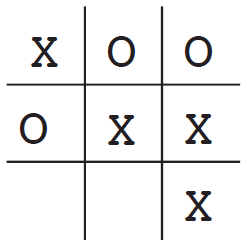
\includegraphics[width=0.25\textwidth]{img/figure_1_tic_tac_toe_board.png}
\end{wrapfigure}
어린 시절 친숙한 틱택토(tic-tac-toe) 게임을 보자. 두 선수는 가로세로 세 칸인
보드에 번갈아 말을 둔다. 한 선수는 X를 다른 선수는 O를 내고, 오른쪽 그림에서
X 선수같이 한쪽이 가로나 세로 혹은 대각선 방향으로 세 칸을 두면 이긴다. 어느
선수도 세 개를 연달아 두지 못하고 칸이 모두 차면 비긴다. 잘 하는 선수는 절대로
안 지도록 말을 둘 수 있기 때문에 우리가 이길 수 있도록 종종 실수하는 불완전한
상대 선수를 가정한다. 여기서는 지거나 비기면 똑같이 안 좋다고 보자. 상대의
약점을 찾고 이길 가능성을 최대화하도록 배우는 선수를 어떻게 만들까?

간단한 문제이지만, 고전적인 방식으로는 만족스럽게 해결하기 쉽지 않다. 예를 들어,
게임이론의 고전적인 ``미니맥스(minimax)'' 방식은 상대가 특이한 식으로 게임을
한다고 가정했기 때문에 여기에 알맞지 않다. 미니맥스 선수라면 조금이라도 질 수
있는 수라면 미숙한 상대 때문에 항상 이길 수 있을지라도 절대로 두지 않는다. 동적
프로그래밍(dynamic programming) 같은 연속 결정 문제를 위한 전통적인 최적화
기법은 어떤 상대에 대한 최적해를 \emph{계산할} 수 있지만, 모든 보드 상태에
상대가 둘 수 확률을 포함하여 상대에 대한 완전한 명세를 입력으로 주어야 한다.
실용적으로 관심이 있는 대부분의 문제와 마찬가지로 이런 정보를 미리 주지 않는다고
가정한다. 한편 상대와 여러 번 게임을 하여 경험을 통해 상대의 정보를 추측할 수
있다. 이 문제에서 아마도 가능한 최선의 방법은 먼저 어느 정도 신뢰할 수 있는
수준까지 상대방 행동 모델을 학습하고 상대의 근사 모델을 가지고 동적 프로그래밍을
적용하여 최적해를 계산하는 것이다. 결국, 이 책에서 다룰 강화학습 기법과 크게
다르지 않다.

이 문제에 진화 기법을 적용하면, 가능한 정책 집합에서 상대방을 이길 확률이 높은
정책을 직접 검색한다. 여기서 정책은 가로세로 세 칸인 보드 위에 X와 O를 조합한
모든 게임 상태마다 선수가 어디에 말을 둘지 알려주는 규칙이다. 정책마다 상대와
일정 횟수 게임을 하여 이길 확률을 추측할 수 있다. 그런 다음 앞으로 무슨 정책을
사용할지 정한다. 전형적인 진화 기법은 계속 정책을 만들고 평가하여 정책 집합에서
정책을 점진적으로 향상한다. 혹은 정책 개체군을 유지하고 평가하는 유전 방식
알고리즘을 사용할 수 있다. 말 그대로 수백 가지 최적화 기법이 가능하다.

가치함수를 사용하여 어떻게 틱택토 문제를 푸는지 보자. 먼저 게임의 모든 상태마다
숫자를 붙인 표를 만든다. 숫자는 가장 최근에 추측한 그 상태에서 승리할 확률이다.
이 추측값을 상태의 \emph{값으로}, 전체 표는 학습한 가치함수로 본다. 현재 A에서
시작하여 승리할 확률이 B에서 시작하는 경우보다 높다고 예측했다면, 상태 A가 상태
B 보다 높은 값을 가진다 혹은 더 ``좋다고'' 말한다. 우리가 항상 X를 둔다면, X가
세 개 줄지어 있는 모든 상태의 승리 확률은 이미 승리했기 때문에 1이다. 비슷한
식으로 O를 세 개 ``채운'' 모든 상태는 우리가 그 상태에서 이길 수 없기 때문에
이길 확률이 0이다. 다른 모든 상태의 초깃값은 이길 확률을 50\%로 짐작하여 0.5로
잡는다.

상대와 여러 번 게임을 한다. 칸을 선택할 때 (비어있는) 둘 수 있는 칸들을 하나씩
채운 상태를 구하고, 표에서 상태들의 현재 값을 찾는다. 대부분의 경우
\emph{탐욕적으로(greedily)} (다른 말로 이길 가능성이 제일 높은) 가장 큰 값을
가진 상태로 이동하는 행동을 선택한다. 그러나 가끔은 무작위로 행동을 선택하기도
한다. 무작위로 선택하지 않으면 절대로 만나지 못할 상태를 경험하기 때문에
\emph{탐색적(exploratory)} 이동이라고 부른다. 게임 중에 고려하고 이동한
움직임들을 그림 \ref{fig:sequence-of-tic-tac-toe-moves}\과 같이 그릴 수 있다.

% page 8

\begin{figure}[h]
\centering
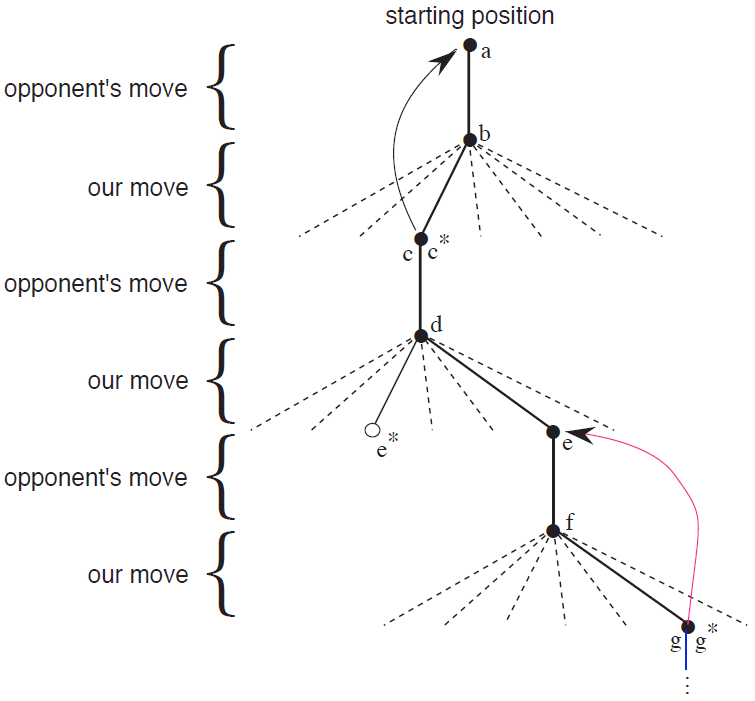
\includegraphics[width=0.5\textwidth]{img/figure_1_sequences_of_tic_tac_toe_moves.png}
\caption{\label{fig:sequence-of-tic-tac-toe-moves}일련의 틱택토 움직임. 게임에서
선택한 움직임은 실선이고, 우리(강화학습 선수)가 고려했지만 선택하지 안은
움직임은 점선으로 표시한다. 두 번째 움직임은 더 우선순위가 높은
e\textsuperscript{$\ast$}로 이어진 길이 옆에 있지만 대신 선택한 탐색적
움직임이다. 탐색적 움직임은 학습하지 않지만, 본문에서 설명하듯이 다른 모든
움직임은 곡선 화살표를 따라 이후 노드에서 이전 노드로 트리를 올라가며 예측값을
갱신한다.}
\end{figure}

게임을 하면서 경험을 통해 상태 값을 변경한다. 그래서 더 정확하게 승리할 확률을
예측하려고 한다. 그림 \ref{fig:sequence-of-tic-tac-toe-moves}의 화살표처럼
탐욕적 움직임을 할 때마다 이동 후 상태 값을 이전 상태로 ``백업(backup)''한다.
정확히는 이전 상태의 현재 값을 이후 상태의 값에 가깝게 갱신한다. 이전 상태의
값을 이후 상태의 값 방향으로 이전 상태의 값을 일정 비율만큼 이동하면 된다.
탐욕적 움직임 이전 상태를 $s$, 이후 상태를 $s'$라고 쓰면, $s$의 예측값 $V(s)$는
다음과 같다.

\begin{equation*}
V(s) \leftarrow V(s) + \alpha[V(s')-V(s)]
\end{equation*}

여기서 $\alpha$는 학습 속도를 조절하는 \emph{스텝 크기 파라미터(step-size
parameter)}라는 작은 양의 분수이다. 이 갱신 규칙은
\emph{시간차(temporal-difference)} 학습 기법의 일종이다. 시간차란 이름은 두 다른
시점의 예측 차이 $V(s') - V(s)$를 기초로 변경하기 때문이다.

위에서 말한 기법은 이 작업에 상당히 적합하다. 예를 들어, 시간이 지나면서 스텝
크기 파라미터를 적절하게 줄인다면,
이 기법은 우리 선수가 모든 상태에서 시작하여 최적의 플레이를 통해 어떤 고정된
상대를 이길 정확한 확률로 수렴한다. 게다가 (탐색적 움직임을 제외하고) 선택한
움직임은 사실 (불완전한) 상대에 대한 최적의 움직임이다. 즉, 상대와 경기하는
최적의 정책으로 수렴한다. 스텝 크기 파라미터가 점차 영으로 줄어들지 않는다면,
이 선수는 자신의 게임 방식을 천천히 바꾸는 선수를 상대로도 잘 싸운다.

% page 9

이 사례는 진화 기법과 가치함수를 학습하는 기법의 차이를 보여준다. 진화 기법은
정책을 평가할 때 정책을 고정한 채 상대와 여러 번 게임을 하거나 상대의 모델을
사용하여 게임을 여러 번 시뮬레이트한다. 승리 빈도는 그 정책으로 승리할 가능성을
공평하게 예측하고, 다음에 어떤 정책을 선택할지 도움을 준. 그러나 여러 번 게임을
한 후에만 정책을 변경하며 오직 게임의 최종 결과만 고려한다. 게임 \emph{과정에서}
일어난 일은 무시한다. 예를 들어, 선수가 이기면 움직임 하나하나가 우승에 얼마나
결정적이었는지 고려하지 않고 게임 중 \emph{모든} 행동이 공을 인정받는다. 심지어
실제로 하지 않은 움직임에도 공이 돌아간다! 반대로 가치함수 기법은 개별 상태를
각각 평가한다. 결국 진화 기법과 가치함수 기법은 모두 정책 집합을 탐색하지만,
가치함수 학습은 경기 과정의 정보를 활용한다.

이 간단한 사례는 강화학습 기법의 몇 가지 핵심 특징을 보여준다. 먼저, 환경과
상호작용하는 학습을 강조한다. 이 경우에서 환경은 상대 선수이다. 두 번째는,
명확한 목표가 있고, 올바로 행동하려면 시간이 흐른 뒤 선택의 효과를 고려한
계획이나 통찰이 필요하다. 예를 들어, 여러 번 움직임으로 근시안적인 상대를
함정으로 몰도록 간단한 강화학습 선수를 학습할 수 있다. 강화학습 해결책은
놀랍게도 상대의 모델을 사용하거나 미래의 모든 상태와 행동을 명시적으로 탐색하지
않고도 계획과 선견지명 효과를 낸다.

이 사례가 몇 가지 강화학습의 핵심 특징을 보여주지만, 사례가 너무 단순해서
강화학습이 제한적이라는 인상을 줄 수 있다. 틱택토는 두 명이 하는 게임이지만,
강화학습은 외부의 적이 없는 경우, 즉 ``자연을 상대로 한 게임''에도 적용할 수
있다. 또한, 강화학습은 틱백토처럼 행동이 에피소드로 구분되고 에피소드가 끝날
때만 보상을 받는 문제에 국한되지 않는다. 행동이 무한히 계속되거나 아무 때나
다양한 보상을 받는 경우도 적용할 수 있다. 틱택토같이 불연속 시간 스텝으로 쪼갤
수 없는 문제도 가능하다. 이론이 더 복잡하기 때문에 이 입문서에서는 다루지
않지만, 연속 시간 문제에도 동일한 원리를 적용할 수 있다.

틱택토는 상태 집합이 상대적으로 작고 유한하지만, 강화학습은 상태가 매우 많거나
심지어 무한대인 경우에도 사용할 수 있다. 예를 들어, 제리
테사우로(\cite{Tesauro1992, Tesauro1995})는 앞에서 말한 알고리즘을 인공신경망과
결합하여 상태가 10\textsuperscript{20}개 정도인 백거먼(backgammon)을 학습했다.
이렇게 상태가 많으면 일부만 경험하기도 불가능하다. 테사우로가 만든 프로그램은
이전 프로그램보다 게임을 훨씬 더 잘 했고, 이제 세계 최고 인간 선수 수준으로
경기한다(\ref{ch:applications-and-case-studies}장 참고). 신경망을 사용한
프로그램은 경험을 일반화할 수 있다. 그래서 새로운 상태에서 신경망은 과거 비슷한
상태의 경험을 토대로 움직임을 선택한다. 강화학습 시스템이 이렇게 상태가 많은
문제를 잘 해결할지는 과거 경험을 적절하게 일반화하는 능력에 달렸다. 그래서
강화학습을 더한 지도학습 기법이 매우 절실하다. 신경망과 딥러닝이
(\ref{sec:nonlinear-function-approximation-artificial-neural-networks}절) 그
방법 중 하나다.

틱택토 예제에서 게임 규칙 외에 아무런 사전 지식 없이 학습을 시작했지만,
강화학습이라고 백지상태에서 출발해서 학습하고 지능을 얻는 것은 아니다. 반대로
다양한 방식으로 강화학습에 사전 지식을 불어넣을 수 있고, 효율적으로 학습할 때
중요할 수 있다. 또한, 여기서는 틱택토 상태를 정확히 알 수 있지만, 강화학습은
일부 상태가 숨겨졌거나 학습자가 보기에 여러 상태가 같아 보이는 경우에도 적용할
수 있다.

% page 10

마지막으로 틱택토 선수는 앞을 내다보고 앞으로 어떤 상태가 나올 수 있는지 알았다.
이를 위해 환경이 해보지 않은 움직임에 어떻게 반응하여 변경할지 ``생각하려면''
게임 모델이 필요하다. 모델이 있는 문제가 많지만, 행동의 영향에 대한 단기 모델도
없는 경우도 있다. 강화학습은 두 경우 모두 적용할 수 있다. 모델이 필요 없지만,
모델이 있거나 모델을 학습할 수 있다면 모델을 쉽게 이용할 수
있다(\ref{ch:planning-and-learning-with-tabular-methods}장).

한편 환경 모델이 전혀 필요 없는 강화학습 기법도 있다. 비모델 시스템은 개별
행동에 대해 환경이 어떻게 반응할지 전혀 생각할 수 수 없다. 상대 측면에서 틱택토
선수는 비모델이다. 상대에 대한 모델이 없기 때문이다. 모델이 유용하려면 어느 정도
정확해야 하기 때문에 충분히 정확한 환경 모델을 만들기 어려운 문제에 막힐 때
복잡한 기법보다 비모델 기법이 유리할 수 있다. 비모델 기법은 모델기반 기법의
중요한 구성요소이기도 하다. 이 책은 여러 장에 걸쳐 비모델 기법을 다룬 다음 더
복잡한 모델기반 기법에서 어떻게 비모델 기법을 사용하는지 볼 것이다.

시스템에서 강화학습을 고수준과 저수준 모두에서 사용할 수 있다. 틱택토 선수는
게임의 기본적인 움직임만 학습하지만, 더 높은 수준에서 각각 ``행동'' 자체가
정교한 문제 풀이 기법인 강화학습도 가능하다. 계층적 학습 시스템은 여러 수준에서
동시에 강화학습을 할 수 있다.

\begin{exercise}[자가 경기(self-play)]
앞에서 설명한 강화학습 알고리즘이 임의의 상대 대신 자기 자신과 경기를 하며 양쪽
모두 학습하는 경우를 가정하자. 어떤 일이 벌어질 것으로 생각하는가? 서로 다르게
움직이는 정책을 학습할까?
\end{exercise}

\begin{exercise}[대칭]
여러 틱택토 칸은 서로 달라 보이지만 대칭 때문에 사실 같다. 이 사실을 활용하여
앞에서 설명한 학습 과정을 어떻게 보완할 수 있을까? 어떤 면에서 학습 과정이
향상되는가? 이제 다시 상대가 대칭을 활용하지 않는 경우를 가정하자. 이 경우
우리는 활용해야 하는가? 만약 활용해야 한다면, 대칭으로 동등한 자리는 반드시
가치가 같아야 하는가?
\end{exercise}

\begin{exercise}[탐욕적인 경기]
강화학습 선수가 \emph{탐욕적이라고}, 즉 항상 가장 가치가 높은 칸을 둔다고
가정하자. 탐욕적이지 않은 선수보다 경기를 잘 하는가 아니면 못하는가? 어떤 문제가
일어날 수 있는가?
\end{exercise}

\begin{exercise}[탐색을 통한 학습]
탐색적 이동을 포함하여 \emph{모든} 움직임마다 학습을 갱신한다고 가정하자. 시간이
지나면서 스텝 크기 파라미터가 적절하게 줄어든다면(그러나 탐색 확률은 줄어들지
않는다), 상태 가치는 어떤 확률에 수렴한다. 탐색적 움직임을 학습한 경우와
학습하지 않은 경우 두 확률은 어떤가? 계속 탐색한다면, 어느 편이 더 잘
학습하는가? 더 많이 이기는 쪽은 어디인가?
\end{exercise}

\begin{exercise}[다른 개선점]
강화학습 선수를 향상할 다른 방법을 생각하자. 여기 틱택토 문제를 더 잘 푸는
방법이 있는가?
\end{exercise}

\section{요약}

강화학습은 계산을 통해 목표 지향 학습과 의사결정을 이해하고 자동화하는 접근
방식이다. 모범을 보이는 감독이나 환경의 완전한 모델에 의존하는 다른 계산적
접근방식과 다르게 강화학습은 환경과 직접 상호작용하는 에이전트의 학습을
강조한다. 우리는 강화학습이 장기 목표를 달성하기 위해 환경과 상호작용을 통해
학습할 때 발생하는 계산 문제를 심각하게 다루는 첫 번째 학문 분야라고 생각한다.

% page 11

강화학습은 학습 에이전트와 환경의 상호작용을 상태와 행동과 보상 형식으로
정의하려고 마르코프 결정 프로세스 형식을 사용한다.
이 구조는 인공지능 문제의 핵심 특징을 단순하게 표현하려고
고안되었다. 인과 관계 개념, 불확실과 비결정론 개념, 명시적인 목표가 존재하는 점
등이 특징이다.

가치와 가치함수 개념은 이 책에서 다루는 대다수의 강화학습 기법의 핵심 특징이다.
우리는 정책 집합을 효율적으로 탐색하는데 가치함수가 중요하다는 입장이다.
강화학습 기법은 가치함수를 사용하기 때문에 전체 정책을 스칼라 평가하여 정책
집합을 직접 탐색하는 진화적 기법과 다르다.

\section{강화학습의 초기 역사}

초기 강화학습의 역사는 두 가지 주된 갈래가 있다. 깊고 풍부한 두 갈래는 현대
강화학습으로 합쳐지기 전에 각자 독립적으로 연구되었다. 한 줄기는 동물 학습
심리학에서 시작한 시행착오를 통한 학습이다. 가장 오래된 인공지능 연구를 거쳐서
1980년대 초 강화학습의 부활로 이어졌다. 다른 줄기는 최적 제어 문제와 가치함수와
동적 프로그래밍을 사용한 최적 제어 풀이이다. 이 갈래는 보통 학습을 다루지
않았다. 두 줄기는 크게 서로 독립적이지만, 이 장의 틱택토 사례에서 사용한 것과
같은 시간차 기법을 다루는 덜 분명한 세 번째 갈래는 예외이다. 1980년대 말 세
줄기가 함께 모여 이 책에 나오는 현대 강화학습 분야가 되었다.

시행착오 학습을 강조한 갈래가 가장 익숙하고 여기서도 주로 다룰 것이다. 그러나 그
전에 최적 제어 갈래를 짧게 언급한다.

``최적 제어(optimal control)''란 용어는 시간에 따른 동적 시스템 행동을
최소화하는 제어기 설계 문제를 설명하려고 1950년대 말에 사용하기 시작했다.
1950년대 중반 리처드 벨만(Richard Bellman) 등이 19세기 해밀턴(Hamilton)과
자코비(Jacobi)의 이론을 확장하여 이 문제의 해결책 중 하나를 만들었다. 이 방법은
동적 시스템 상태와 가치함수 혹은 ``최적 이익 함수'' 개념을 사용하여 지금은 벨만
방정식(Bellman equation)이라고 부르는 함수식을 정의한다. 이 방정식을 가지고 최적
제어 문제를 푸는 기법을 동적 프로그래밍(\cite{Bellman1957a})이라고 부르게 된다.
또, 벨만(\cite*{Bellman1957b})은 마르코프 결정 프로세스(Markovian decision
processe, MDP)이라는 최적 제어 문제의 이산 확률 버전을 소개했고, 로널드
하워드(\cite{Howard1960})는 MDP를 위한 정책 반복법(policy iteration method)을
고안했다. 이것들은 현대 강화학습 이론과 알고리즘의 근간이 되는 핵심 요소이다.

동적 프로그래밍은 일반적인 확률 최적 제어 문제의 유일한 풀잇법으로 널리
알려졌다. 동적 프로그래밍은 벨만이 말한 (상태 변수 개수가 증가할 때 계산량이
지수적으로 증가하는) ``차원의 저주''에 시달리지만, 다른 일반적인 기법보다 여전히
훨씬 더 효율적이고 폭넓게 적용할 수 있다. 동적 프로그래밍은 1950년대 후반부터
부분 관찰 MDP(\cite{Lovejoy1991}), 여러 가지 응용(\cite{White1985, White1988,
White1993}), 근사 기법(\cite{Rust1996}), 비동기 기법(\cite{Bertsekas1982,
Bertsekas1983}) 등으로 널리 연구되었다. 여러 훌륭한 현대 동적 프로그래밍 교재가
있다(\cite[예,][]{Bertsekas2005, Bertsekas2012, Puterman1994, Ross1983,
Whittle1982, Whittle1983}). 브라이슨(\cite{Bryson1996})은 최적 제어 분야의
역사를 충실하게 알려준다.

최적 제어와 동적 프로그래밍 (그리고 학습) 사이의 관계는 느리게 파악되었다.
거리를 둔 원인은 확신할 수 없지만, 연관 분야가 차이 났고 목표가 달랐기 때문일
것이다. 동적 프로그래밍을 기본적으로 정확한 시스템 모델과 벨만 방정식의 해석적
풀이에 의존한 오프라인 계산으로 본 팽배한 시각도 한몫했을 것이다. 게다가 가장
단순한 형태의 동적 프로그래밍은 과거 방향으로 계산을 진행하기 때문에 미래
방향으로 진행해야 하는 학습 과정에 적용하기 힘들었다. 벨만과
드레퓌스(\cite{BellmanDreyfus1959}) 같은 일부 동적 프로그래밍 초기 연구는 학습
접근 방식을 따른다고 분류할 수 있다. (뒤에 나오는) 위튼의
연구(\cite{Witten1977})는 확실히 학습과 동적 프로그래밍 개념이 섞여 있다.
워보스(\cite{Werbos1987})는 동적 프로그래밍과 학습 기법의 상관관계가 중요하고 이
관계가 신경과 인지 동작 방식을 이해하는 데 도움이 된다고 주장했다. 1989년 크리스
왓킨의 연구는 동적 프로그래밍 기법과 온라인 학습의 완전히 결합했고, MDP 형식의
강화학습 연구가 널리 퍼졌다(\cite{Watkins1989}). 이후 여러 연구자가 이 관계를
중점적으로 발전시켰다. 특히 드미트리 베르트세카스와 존
치치클리스(\cite{BertsekasTsitsiklis1996})는 동적 프로그래밍과 신경망을 결합하여
``신경역동 프로그래밍''이란 말을 만들었다. 현재는 ``근사 동적
프로그래밍(approximate dynamic programming)''이란 용어를 사용한다. 이런 다양한
접근 방식은 주제의 다른 측면을 강조하지만, 모두 강화학습처럼 동적 프로그래밍의
전통적인 단점을 회피하는 데 관심이 있다.

% page 12

우리는 모든 최적 제어 기법은 어떤 의미에서 강화학습에도 가능하다고
본다. 우리는 강화학습 문제를 효율적으로 푸는 모든 방법을 강화학습 기법으로
정의한다. 그리고 강화학습 문제는 최적 제어 문제와 (특히 MDP로 기술할 수 있는
확률 최적 제어 문제와) 밀접하게 연관이 있다. 따라서 동적 프로그래밍 같은 최적
제어 풀잇법을 강화학습 기법으로 봐야 한다. 거의 모든 전통적인 기법은 제어하는
시스템을 완벽하게 알아야 하기 때문에 강화학습의 일부라고 말하기에 조금
부자연스럽다. 그러나 많은 동적 프로그래밍 알고리즘은 점진적이고 반복적이다. 학습
기법 같이 계속 근사하여 올바른 답에 도달한다. 앞으로 보겠지만 단지 겉모습만
비슷하지 않고 훨씬 근본적으로 유사하다. 완전한 지식과 불완전한 지식에 대한
이론과 해법은 너무 밀접하게 연관되었기 때문에 한 가지 주제의 일부로 함께
고려해야 한다고 생각한다.

이제 시행착오 학습 개념을 따르는 현대 강화학습을 이끈 다른 갈래로 돌아가자.
여기서는 중요한 점만 언급하고 \ref{ch:psychology}장에서 자세히 다룰 것이다.
미국의 심리학자 우드워스에 따르면, 시행착오 학습 개념은 1850년대 알렉산더
베인(Alexander Bain)의 ``암중모색과 실험''에 의한 학습까지 거슬러 가고, 더
직접적으로는 1894년 영국의 동물행동학자 겸 심리학자 콘웨이 로이드 모간(Conway
Lloyd Morgan)이 관찰한 동물 행동을 설명할 때 이 용어를
사용했다(\cite{Woodworth1938}). 시행착오 학습이 학습 원리의 핵심이라고 처음으로
말한 사람은 아마도 에드워드 손다이크이다.

\begin{displayquote}
동일한 상황에서 동물이 즉시 만족하거나 곧 만족하게 되는 반응은, 다른 조건이
동일하다면, 상황과 더 강하게 연결된다. 그래서 상황이 반복하면, 반응이 반복할
가능성이 높아진다. 동물이 싫어하거나 곧 싫게 되는 반응은, 다른 조건이
동일하다면, 환경과 연관이 약해진다. 그래서 반복할수록 일어날 가능성이 낮아진다.
만족이나 불쾌함이 커질수록 연결이 강해지거나 약해진다.
(\cite[p.~244]{Thorndike1911})
\end{displayquote}

강화하는 사건이 행동 선택 경향에 미치는 영향을 보여주기 때문에 손다이크는 이것을
``효과의 법칙(Law of Effect)''이라고 불렀다. 이후 손다이크는 (보상과 체벌의 효과
차이 같은) 동물 학습에 대한 축적된 자료를 더 잘 설명하도록 법칙을 변경했고,
다양한 형태의 법칙이 학습 이론가 사이에서 상당히 논란이
되었다(\cite[예,][참고]{Gallistel2005, Herrnstein1970, Kimble1961, Kimble1967,
Mazur1994}). 논란에도 불구하고 한두 가지 형태의 효과의 법칙은 대부분 행동의
근간이 되는 기본 원리로 널리 인정받았다(\cite[예,][]{HilgardBower1975,
Dennett1978, Campbell1960, Cziko1995}). 클라크 헐의 영향력있는 학습 이론과
스키너의 실험 기법의 기초가 된다(\cite[예,][]{Hull1943, Skinner1938}).

% page 13

손다이크가 효과의 법칙을 말한 이후 동물 학습 분야에서 ``강화''란 용어를 널리
사용했고, 우리가 알기로는 파블로프(Pavlov) 조건반사 논문의 1927년 영어 번역에서
이런 의미로 처음 등장한다.  강화는 다른 자극 혹은 응답과 적절한 시간 관계를 가진
자극(강화물, reinforcer)을 받은 동물의 행동 패턴 강화이다. 일부 심리학자는
강화는 물론이고 약화 과정까지, 즉 사건의 생략이나 중단이 행동을 변화하는 경우를,
포함하도록 이 의미를 확장한다. 강화는 행동을 변화하고, 강화물이 사라져도 변화한
행동을 지속시킨다. 그래서 지속되는 변화 없이 동물의 관심을 끌거나 행동을
격려하는 자극은 강화물로 보지 않는다.

인공지능의 가능성에 대한 초기 발상 중에 컴퓨터로 시행착오 학습을 구현하는
아이디어가 나왔다. 앨런 튜링은 1948년 보고서에서 효과의 법칙의 연장선에서
``쾌락-고통 시스템(pleasure-pain system)'' 설계를 다루었다.

\begin{displayquote}
무슨 행동을 할지 결정하지 않은 배치에 도달하면, 없는 데이터 자리에 임의로 선택한
적절한 항목을 기록하고 시험 삼아 적용한다. 고통 자극이 발생하면 모든 시험적
항목을 취소하고, 기쁨 자극이 발생하면 모두 그대로 둔다. (\cite{Turing1948})
\end{displayquote}

시행착오 학습을 보여주려고 많은 독창적인 전기기계 장치가 만들어졌다. 가장 초기
장치는 토마스 로스(\cite{Ross1933})가 만든 간단한 미로를 통과하며 스위치
설정으로 길을 기억하는 기계였다. 1951년에는 이미 ``기계 거북이''로 알려진 그레이
월터(\cite{Walter1950})가 단순한 학습이 가능한 거북이를
만들었다(\cite{Walter1951}). 1952년 클로드 섀넌은 시행착오를 통해 길을 찾는
테세우스(Theseus)라는 미로 찾기 쥐를 선보였다. 미로는 바닥 아래에 있는 자석과
릴레이를 가지고 성공한 방향을 기억했다(\cite{Shannon1951, Shannon1952}).
도이치(\cite{Deutsch1954})는 어떤 면에서 모델기반
강화학습(\ref{ch:planning-and-learning-with-tabular-methods}장)과 유사한 자신의
행동 이론(\cite{Deutsch1953})에 기반을 둔 미로 찾기 장치를 설명했다. 마빈
민스키는 박사 논문(\cite{Minsky1954})에서 강화 학습의 계산 모델과 함께 두뇌의
변경 가능한 시냅스 연결을 (\ref{ch:neuroscience}장) 흉내낸 SNARCs(Stochastic
Neural-Analog Reinforcement Calculators)라는 구성요소로 만든 아날로그 장치를
설명했다. 멋진 웹사이트 \url{cyberneticzoo.com}에 이런 전기기계 학습 장치에
대한 정보가 풍부하다.

전기기계 학습 장치 제작은 시행착오 학습을 포함하여 다양한 종류의 학습을 수행하는
프로그래밍 디지털 컴퓨터로 이어졌다. 팔리와 클라크(\cite{FarleyClark1954})는
시행착오를 통해 학습하는 신경망 학습 기계를 디지털 시뮬레이션했다. 그러나 그들은
곧 관심을 시행착오 학습에서 일반화와 패턴인식으로, 즉 강화학습에서 지도학습으로
옮겼다(\cite{ClarkFarley1955}). 이렇게 학습 종류들의 관계를 혼동하기 시작했다.
많은 연구자이 사실은 지도학습을 연구하지만 자신은 강화학습을 연구한다고 믿곤
했다. 예를 들어, 신경망을 개척한 로젠블렛(\cite{Rosenblatt1962}) 그리고 위드로와
호프(\cite{WidrowHoff1960})는 보상과 체벌이란 언어를 사용하는 등 분명히
강화학습에서 영감을 받았지만, 패턴인식과 지각학습에 적합한 지도학습 시스템을
연구했다. 심지어 오늘날에도 일부 연구자와 교과서는 학습 종류들의 구분을
최소화하거나 모호하게 만든다. 예를 들어, 일부 신경망 교과서는 훈련 예제를 가지고
학습한 망을 설명할 때 ``시행착오''란 단어를 사용한다. 망이 연결 가중치를
갱신하려고 오류 정보를 사용하기 때문에 혼동이 이해되지만, 어떤 행동이 올바른지
알지 않고 피드백을 평가하여 행동을 선택하는 시행착오 학습의 핵심 특징을
간과한다.

% page 14

% correction: McClaren -> McLaren
어느 정도는 이런 혼동 때문에 몇 가지 주목할만한 예외를 제외하고는 1960년대와
1970년대에 순수한 시행착오 학습 연구가 드물었다. 1960년대에 시행착오 학습의
공학 사례를 다루며 공학 논문에서 ``강화''와 ``강화학습''이란 용어가 처음
등장한다(\cite[예,][]{WaltzFu1965, Mendel1966, Fu1970, MendelMcLaren1970}). 특히
민스키의 영향력 있는 ``인공지능을 향한 단계(Steps Toward Artificial
Intelligence)'' 논문(\cite{Minsky1961})은 예측과 기대 그리고 그의 표현에 따르면
\emph{복잡한 강화학습 시스템을 위한 기본 크레디트-할당 문제} (성공 크레디트를
분배하는 방법) 등 시행착오 학습의 여러 쟁점을 다룬다. 이 책에서 다루는 모든
기법은 어떤 의미에서 이 문제를 풀려고 한다. 민스키의 논문은 지금도 읽을 가치가
있다.

이제 1960년대와 1970년대 계산적이고 이론적인 순수 시행착오 학습 연구와 거리가
있는 몇 가지 예외를 보자.

그중 하나는 존 안드레라는 뉴질랜드 연구자의 연구이다.
안드레(\cite{Andreae1963})는 환경과 상호작용하며 시행착오를 통해 학습하는 STeLLA
시스템을 개발했다. 이 시스템은 숨겨진 상태 문제를 다루기 위해 세상의 내부 모델을
가진다(\cite{Andreae1969a}). 내부 모델은 나중에 ``내부 독백''이라고 불렀다.
안드레의 이후 연구(\cite*{Andreae1977})는 교사로부터 학습을 더 강조하지만,
시스템 목표 중 하나로 새로운 사건을 발생하고 여전히 시행착오를 통한 학습이 있다.
우리가 말한 백업 갱신 작업과 유사한 크레디트-할당 방식을 구현한 ``리크백
프로세스''가 이 연구의 특징이었다. 안드레는 책(\cite*{Andreae1998})에서 리크백
프로세스를 더 자세히 설명한다.
불행하게도 그의 선구적인 연구는 잘 알려지지 않았고,
이후 강화학습 연구에 큰 영향을 주지 않았다.

도널드 미치(Donald Michie)의 연구는 더 영향력이 있었다. \cite*{Michie1961}년과
\cite*{Michie1963}년 그는 틱택토 게임을 하는 방법을 학습하는 간단한 시행착오
학습 시스템 MENACE(Matchbox Educable Naughts and Crosses Engine)를 공개했다.
모든 게임 칸마다 성냥갑이 있고, 성냥갑에는 그 자리에서 움직일 수 있는 칸마다
다른 색으로 색칠한 알들이 들어있다. 현재 게임 칸에 해당하는 성냥갑에서 무작위로
알을 뽑아서 MENACE 움직임을 결정한다. 게임이 끝나면 MENACE 결정을 강화하거나
체벌하기 위해 게임에 사용한 알들을 성냥갑에 추가하거나 제거한다. 미치와
챔버스(\cite{MichieChambers1968})는 GLEE(Game Learning Expectimaxing Engine)라는
또 다른 틱택토 강화학습기와 BOXES라는 강화학습 제어기도 소개했다. 그들은
움직이는 카트로 막대의 균형을 잡는 학습에 BOXES를 적용했다. 막대가 쓰러지거나
카트가 선로 끝에 다다를 때만 실패 신호가 발생한다. 막대의 균형을 잡을 수 있는
교사가 설명한다고 가정한 지도학습 기법을 사용한 위드로와
스미스(\cite{WidrowSmith1964})의 앞선 연구를 변형한 것이다. 미치와 챔버스의
막대균형잡이는 불완전한 지식 조건에서 강화학습의 가장 훌륭한 초기 사례 중
하나다. 우리 연구(\cite{BartoSuttonAnderson1983, Sutton1984})를 시작으로 이후
강화학습 연구에 큰 영향을 미쳤다. 미치는 꾸준하게 시행착오와 학습이 인공지능에서
없어서는 안된다고 강조한다(\cite{Michie1974}).

위드로와 굽타와 마이트라(\cite{WidrowGuptaMaitra1973})는 위드로와
호프(\cite{WidrowHoff1960})의 최소 제곱 평균(LMS) 알고리즘을 변경하여 훈련 예제
대신 성공과 실패 신호를 학습할 수 있는 강화학습 규칙을 만들었다. 그들은 이 학습
형태를 ``선택적 부트스트랩 적응''이라고 부르고, ``교사와 학습''이 아니라
``비평가와 학습''이라고 표현했다. 이 규칙을 분석하여 블랙잭을 어떻게 배우는지
보여주었다. 지도학습에 엄청난 기여를 한 위드로가 강화학습에 관여한 사례이다.
``비평가(critic)''란 단어는 위드로, 굽타, 마이트라 논문에서 유래했다. 이와
무관하게 뷰캐넌, 미첼, 스미스, 존슨(\cite{BuchananMitchellSmithJohnson1978})은
기계학습 맥락에서 비평가란 단어를 사용했지만
(\cite[또,][참고]{DietterichBuchanan1984}), 여기서는 성능 평가 이상의 일을 할 수
있는 전문가 시스템을 뜻한다.

% page 15

\emph{학습 오토마타} 연구는 현대 강화학습 연구로 이어지는 시행착오 갈래에 더
직접적인 영향을 미쳤다. \emph{k 암드 밴디트(k-armed bandit)}로 알려진 비연합이고
순수하게 선택적인 학습 문제를 푸는 기법들이다(\ref{ch:multi-armed-bandits}장).
k 암드 밴디트는 ``한 손 강도(one-armed bandit)'', 즉, 손잡이가 $k$개인
슬롯머신을 비유한 말이다. 학습 오토마타는 이런 문제에서 보상 확률을 향상하는 큰
메모리가 필요 없는 단순한 기계이다. 학습 오토마타는 러시아의 수학자이자
물지학자인 짜이틀린(Tsetlin)과 동료들의 1960년대 연구(짜이틀린 사후에 출판됨,
\cite*{Tsetlin1973})에서 유래하였고, 그 후 공학에서 집중적으로
발전했다(\cite[참고]{NarendraThathachar1974, NarendraThathachar1989}). 보상
신호를 기초로 행동 확률을 갱신하는 방법인 \emph{확률 학습 오토마타} 연구도 그중
하나다. 확률 학습 오토마타에 앞서 심리학에서는 1950년 윌리엄 에스테스가 학습의
확률적 이론(\cite{Estes1950})을 연구하기 시작했고, 심리학자 로버트 부시와
통계학자 프레데릭 모스텔라(\cite{BushMosteller1955}) 등이 더 발전시켰다.

심리학에서 개발된 확률적 학습 이론을 경제학자들이 채택하여 경제학 분야에서
강화학습 연구로 이어졌다. 이 작업은 1973년 부시와 모스텔라 학습 이론을 고전 경제
모델들에 적용하면서 시작했다(\cite{Cross1973}). 연구의 목표는 전통적인 이상적
경제 에이전트가 아니라 실제 사람 같이 행동하는 인공 에이전트
탐구다(\cite{Arthur1991}). 이 접근 방식은 게임이론 영역에서 강화학습 연구로
커졌다. 경제학의 강화학습은 인공지능의 초기 연구와 무관하게 발전했지만,
강화학습과 게임이론은 현재 두 분야의 공통 관심 주제이다. 그러나 이 내용은 이
책의 범위를 넘어선다. 캐머러(\cite{Camerer2003})는 경제학의 강화학습 전통을
들려주며 노웨 등(\citeauthor*{NoweVrancxHauwere2012},
\cite*{NoweVrancxHauwere2012})은 이 책에서 소개하는 접근 방식을 다중 에이전트로
확장한 관점에서 주제를 개관한다. 게임이론 관점의 강화는 틱택토나 체커처럼 즐기는
게임을 플레이하는 프로그램에서 사용하는 강화학습과 매우 다른 주제다. 예를 들어,
지타(\cite{Szita2012})는 이런 강화학습과 게임 측면을 소개한다.

% correction: Walsh, 1996, and Koza, 1992 -> Walsh, 1996; Koza, 1992
존 홀랜드(\cite{Holland1975})는 선택적 원칙에 기반한 일반 적응 시스템 이론을
시작한다. 그는 초기에 진화 기법과 $k$ 암드 밴디트의 비연합 형태 시행착오를 주로
연구했다. 1976년과 1986년에 들어 연합과 가치 함수를 포함한 진정한 강화학습
시스템인 \emph{분류기 시스템}을 소개했다. 홀랜드의 분류기 시스템의 핵심
구성요소는 (틱택토 사례에서 사용한 시간차 알고리즘과 밀접하게 관련되고
\ref{ch:temporal-difference-learning}장에서 다룰) 크레디트 할당을 위한 ``물통
릴레이 알고리즘''이었다. 다른 핵심 구성요소는
\emph{유전 알고리즘}이었다. 유전 알고리즘으로 유용한 표현형을
진화시켰다. 여러 연구자가 분류기 시스템을 널리 개발하여 강화학습의 주된 연구
분야가 되었지만(\cite{UrbanowiczMoore2009}), 진화적 컴퓨팅의 다른 접근 방식과
마찬가지로 (우리는 그 자체로 강화학습이라고 여기지 않는) 유전자 알고리즘은 훨씬
많은 관심을 받았다(\cite[예,][]{FogelOwensWalsh1966, Koza1992}).

시행착오 갈래를 인공지능 분야의 강화학습으로 되살린 최대 수훈자는 핸리
클로프이다(\cite{Klopf1972, Klopf1975, Klopf1982}). 클로프는 학습 연구자들이
거의 지도학습만 몰두하여 적응 행동의 본질적인 측면이 간과되었다고 생각했다.
클로프는 행동의 쾌락 측면, 환경에서 어떤 결과를 얻으려는 동기, 바라는 목적을
지향하고 원하지 않는 목적을 지양하는 환경 제어가 빠졌다고 보았다. 이들은
시행착오 학습의 핵심 개념이다. 이점이 지도학습과 강화학습을 구별하고 결국
강화학습에 집중하도록 도와주었기 때문에(\cite{BartoSutton1981a}) 클로프의 발상은
저자들에게 특히 큰 영향을 주었다. 우리 동료들이 이룬 많은 초기 성과는 강화학습이
지도학습과 다름을 보이는 방향이었다(\cite{BartoSuttonBrouwer1981,
BartoSutton1981b, BartoAnandan1985}). 강화학습이 신경망 학습의 중요한 문제를,
특히 다층망 학습 알고리즘 생성 방법을, 처리할 수 있다는 연구도
있다(\cite{BartoAndersonSutton1982, BartoAnderson1985, BartoAnandan1985,
Barto1985, Barto1986, BartoJordan1987}). 강화학습과 신경망은
\ref{ch:neuroscience}장에서 더 다룰 것이다.

% page 16

이제 강화학습 역사의 세 번째 갈래인 시간차 학습을 살펴보자. 시간차 학습 기법은
틱택토 승리 확률 같은 어떤 양을 예측하고 시간상 연속된 예측값의 차이로 동작하는
점이 특징이다. 이 갈래는 다른 두 갈래보다 작고 덜 뚜렷하지만, 시간차 기법이
새롭고 강화학습에 고유하다는 등의 이유로 강화학습에서 특히 중요한 역할을 했다.

시간차 학습은 어느 정도는 동물 학습 심리학, 특히 \emph{이차적 강화자극(secondary
reinforcer)} 개념에서 나왔다고 할 수 있다. 이차적 강화자극은 음식과 고통 같은
일차적 강화자극과 쌍을 이루는 자극으로, 결과적으로 강화 성질이 비슷하다. 아마도
민스키(\cite*{Minsky1954})가 이 심리 이론이 인공 학습 시스템에 중요할 수 있다고
처음 발견했을 것이다. 아더 사무엘(\cite{Samuel1959})은 그의 유명한 체커 게임
프로그램에서 처음으로 시간차 개념을 가진 학습 기법을 제안하고 구현했다.

사무엘은 민스키의 연구나 동물 학습과 관계를 언급하지 않았다. 분명히 그는 평가
함수를 사용하여 컴퓨터가 체스를 두도록 프로그래밍할 수 있고 실행 중에 평가
함수를 변경하여 경기력을 향상할 수 있다는 클로드 섀넌(\cite*{Shannon1950})의
제안에서 영감을 받았다. (벨만도 섀넌의 아이디어의 영향을 받았을지도 모르지만
증거는 없다.) 민스키(\cite*{Minsky1961})는 자신의 ``단계'' 논문에서 자연과 인공
모두에서 이차 강화 이론과 연관성을 시사하며 사무엘의 연구를 크게 다루었다.

말했듯이 민스키와 사무엘의 연구 이후 십 년간 시행착오 학습에 대한 계산 연구가
거의 없었고, 시간차 학습 연구는 전무했다. \cite*{Klopf1972}년 클로프는 시간차
학습의 중요한 요소와 함께 시행착오 학습을 제시했다. 클로프는 학습을 큰
시스템으로 확장할 수 있는 원리에 관심을 가지고, 전체 학습 시스템의 부분들이
서로를 강화하는 지역 강화 개념에 매료되었다. 그는 모든 요소(즉, 모든 뉴런)가
모든 입력을 흥분 입력은 보상으로 억제 입력은 체벌로 해석하는 ``일반화된 강화''
개념을 만들었다. 현재 시간차 학습과 개념이 다르고, 뒤돌아 생각해보면 사무엘의
연구보다 더 나아갔다. 한편 클로프는 이 개념을 시행착오 학습과 결합하고, 동물
학습 심리학의 방대한 경험과 관련시켰다.

서튼(\cite*{Sutton1978a, Sutton1978b, Sutton1978c})은 클로프의 발상을, 특히 동물
학습 이론과 연결하여 더 발전시켜서 시간상 연속한 예측의 변화로 학습 규칙을
설명했다. 서튼과 바토는 이 발상을 다듬어서 시간차 학습에 기반을 둔 고전적 조건
형성 심리학 모델을 만들었다(\cite{SuttonBarto1981a, BartoSutton1982}). 그 후
시간차 학습을 사용한 몇 가지 다른 유력한 고전적 조건 형성 심리학 모델도
나왔다(\cite{Klopf1988, MooreEt1986, SuttonBarto1987, SuttonBarto1990}). 대부분
역사적 관련이 없지만, 이 시기에 나온 몇 가지 신경과학 모델도 시간차 학습
입장에서 잘 해석된다(\cite{HawkinsKandel1984, ByrneGingrichBaxter1990,
GelperinHopfieldTank1985, Tesauro1986, FristonEt1994}).

우리의 초기 시간차 학습 연구는 동물 학습 이론과 클로프의 연구에 큰 영향을
받았다. 민스키 ``단계'' 논문과 사무엘의 체커 게임기와 관계는 시간이 흐른 후에야
알게 되었다. 그러나 1981년 무렵에 우리는 앞에서 언급한 모든 선행 연구를 시간차와
시행착오 갈래로 인식하게 되었다. 그 시기에 우리는 시간차 학습을 시행착오 학습과
결합하여
사용한 \emph{액터-크리틱 아키텍처(actor-critic architecture)} 기법을 만들고,
미치와 챔버스의 막대 균형 문제에 적용했다(\cite{BartoSuttonAnderson1983}). 이
기법은 서튼의 박사 논문(\cite*{Sutton1984})에서 집중적으로 다루었고, 앤더슨의
박사 논문(\cite*{Anderson1986})은 역전파 신경망을 사용하여 확장했다. 그 무렵
홀랜드(\cite*{Holland1986})는 시간차 아이디어를 물통 릴레이 알고리즘 형태로 그의
분류기 시스템에 직접
도입했다. 중요한 사건은 \cite*{Sutton1988}년 서튼이 시간차 학습을 제어와
구분하여 일반 예측 기법으로 취급한 점이다. 그 논문은 TD($\lambda$) 알고리즘을
소개하고 일부 수렴 조건을 증명하기도 했다.

% page 17

1981년 액터-크리틱 아키텍처 연구를 마무리할 때 우리는 시간차 학습 규칙을 가장
먼저 수록했다고 보이는 이언 위튼(\cite{Witten1977})의 논문을 발견했다. 그는
MDP를 푸는 적응 제어기의 일부로 우리가 표 TD(0)이라고 부르는 기법을 제안했다.
위튼의 연구는 안드레의 초기 STeLLA 실험과 다른 시행착오 학습 시스템을 계승했다.
그래서 위튼의 1977년 논문은 시간차 학습에 독특한 초기 기여이며 동시에 강화학습
연구의 주된 갈래(시행착오 학습과 최적 제어)를 모두 아우른다.

시간차와 최적 제어 갈래는 \cite*{Watkins1989}년 크리스 왓킨이 Q-학습을
개발하면서 완전히 결합한다. 이 연구는 세 강화학습 연구 갈래의 이전 연구를
확장하고 통합한다. 폴 워보스(\cite{Werbos1987})는 \cite*{Werbos1977}년부터
시행착오 학습과 동적 프로그래밍의 수렴을 주장하며 통합에 일조했다. 왓킨이
연구하던 시절 강화학습 연구가 엄청나게 성장했다. 특히 인공지능의 기계학습 분야가
성장했지만, 신경망과 인공지능도 폭넓게 발전했다. 1992년 제리 테사우로의 백거먼
게임 프로그램 TD-Gammon의 놀라운 성공은 이 분야에 더 관심을 일으켰다.

이 책 초판 출판 이후 강화학습 알고리즘과 신경 시스템의 강화학습 사이의 관계를
주목한 신경과학의 하위분야가 번창했다. 여러 연구자가 지적했듯이 시간차
알고리즘의 행동과 뇌에서 도파민을 생성하는 뉴런의 동작이 신기할 정도로 비슷한
점이 그 이유이다(\cite{FristonEt1994, Barto1995a, HoukAdamsBarto1995,
MontagueDayanSejnowski1996, SchultzDayanMontague1997}).
\ref{ch:neuroscience}장은 강화학습의 이런 흥미로운 측면을 소개한다.

최근 강화학습 역사에 중요한 기여가 너무 많아서 이 짧은 글에 다 언급할 수 없다.
일부는 관련 장 마지막에 인용한다.

\section*{참고문헌}

% correction: Wering -> Wiering
강화학습 일반은 \textcite{Szepesvari2010}, \textcite{BertsekasTsitsiklis1996},
\textcite{Kaelbling1993a}, Sugiyama et al.
(\cite*{SugiyamaHachiyaMorimura2013}) 책을 참고하라. Si et al.
(\cite*{SiBartoPowellWunsch2004}), \textcite{Powell2011},
\textcite{LewisLiu2012}, \textcite{Bertsekas2012} 책은 제어 혹은 운용 과학
관점을 취한다. \textcite{Cao2009}는 확률 동적 시스템의 학습과 최적화에 대한 다른
접근 방식으로서 강화학습을 다룬다. 《Machine Learning》 저널
\textcite{Sutton1992}, \textcite{Kaelbling1996}, \textcite{Singh2002}은 강화학습
특별호다. \textcite{Barto1995b}, \textcite{KaelblingLittmanMoore1996},
\textcite{KeerthiRavindran1997}의 개론도 유용하다.
\textcite{WieringVanOtterlo2012}가 편집한 책은 최근 발전을 잘 개관한다.

\begin{description}[labelsep=2em]

\item[1.2]
이 장에 나오는 필의 아침 예는 \textcite{Agre1988}에서 영감을 받았다.

\item[1.5]
틱택토 사례에서 사용한 시간차 기법은 \ref{ch:temporal-difference-learning}장에서
다룬다.

\end{description}



\part{Tabular Solution Methods}\label{pt:tabular-solution-methods}

\chapter{Multi-armed Bandits}\label{ch:multi-armed-bandits}

\chapter{Finite Markov Decision Processes}\label{ch:finite-markov-decision-processes}

\chapter{Dynamic Programming}\label{ch:dynamic-programming}
\section{Policy Evaluation (Prediction)}
\section{Policy Improvement}\label{sec:policy-improvement}
\section{Policy Iteration}
\section{Value Iteration}
\section{Asynchronous Dynamic Programming}
\section{Generalized Policy Iteration}\label{sec:generalized-policy-iteration}


\chapter{몬테카를로 기법}\label{ch:monte-carlo-methods}

\begin{equation*}
\pi_0 \xrightarrow{\hspace{0.4em}\text{E}\hspace{0.4em}} q_{\pi_0} \xrightarrow{\hspace{0.4em}\text{I}\hspace{0.4em}}
 \pi_1 \xrightarrow{\hspace{0.4em}\text{E}\hspace{0.4em}} q_{\pi_1} \xrightarrow{\hspace{0.4em}\text{I}\hspace{0.4em}}
 \pi_2 \xrightarrow{\hspace{0.4em}\text{E}\hspace{0.4em}} \cdots \xrightarrow{\hspace{0.4em}\text{I}\hspace{0.4em}}
 \pi_\ast \xrightarrow{\hspace{0.4em}\text{E}\hspace{0.4em}} q_\ast
\end{equation*}

\begin{equation}
\pi(s) \doteq \argmax_a q(s,a).
\end{equation}

\begin{align*}
q_{\pi_k}(s,\pi_{k+1}(s)) &= q_{\pi_k}(s,\argmax_a q_{\pi_k}(s,a)) \\
 &= \max_a q_{\pi_k}(s,a) \\
 &\geq q_{\pi_k}(s,\pi_k(s)) \\
 &\geq v_{\pi_k}(s).
\end{align*}

\begin{align}
q_\pi(s,\pi'(s)) &= \sum_a \pi'(a|s)q_\pi(s,a) \nonumber\\
 &= \frac{\epsilon}{|\mathcal{A}(s)|} \sum_a q_\pi(s,a) + (1-\epsilon)\max_a q_\pi(s,a) \\
 &\geq \frac{\epsilon}{|\mathcal{A}(s)|} \sum_a q_\pi(s,a) + (1-\epsilon)\sum_a \frac{\pi(a|s) - \frac{\epsilon}{|\mathcal{A}(s)|}}{1-\epsilon}q_\pi(s,a) \nonumber
\intertext{(the sum is a weighted average with nonnegative weights summing to 1,
 and as such it must be less than or equal to the largest number averaged)}
 &= \frac{\epsilon}{|\mathcal{A}(s)|} \sum_a q_\pi(s,a) - \frac{\epsilon}{|\mathcal{A}(s)|} \sum_a q_\pi(s,a) + \sum_a \pi(a|s)q_\pi(s,a) \nonumber\\
 &= v_\pi(s). \nonumber
\end{align}

\begin{align*}
\tilde{v}_\ast(s) &= (1-\epsilon)\max_a \tilde{q}_\ast(s,a) + \frac{\epsilon}{|\mathcal{A}(s)|} \sum_a \tilde{q}_\ast(s,a) \\
 &= (1-\epsilon)\max_a \sum_{s',r} p(s',r|s,a) \Big[r+\gamma\tilde{v}_\ast(s')\Big] \\
 &\qquad + \frac{\epsilon}{|\mathcal{A}(s)|} \sum_a \sum_{s',r} p(s',r|s,a) \Big[r+\gamma\tilde{v}_\ast(s')\Big].
\end{align*}



\chapter{Temporal-Difference Learning}\label{ch:temporal-difference-learning}

\chapter{$n$-step Bootstrapping}\label{ch:n-step-bootstrapping}

\chapter{Planning and Learning with Tabular Methods}\label{ch:planning-and-learning-with-tabular-methods}

\part{Approximate Solution Methods}\label{ch:approximate-solution-methods}

\chapter{On-policy Prediction with Approximation}\label{ch:on-policy-prediction-with-approximation}
\section{Value-function Approximation}
\section{The Prediction Objective (\textoverline{VE})}
\section{Stochastic-gradient and Semi-gradient Methods}
\section{Linear Methods}
\section{Feature Construction for Linear Methods}
\section{Nonlinear Function Approximation: Artificial Neural Networks}\label{sec:nonlinear-function-approximation-artificial-neural-networks}

\chapter{On-policy Control with Approximation}\label{ch:on-policy-control-with-approximation}

\chapter{*Off-policy Methods with Approximation}\label{ch:off-policy-methods-with-approximation}

\chapter{Eligibility Traces}\label{ch:eligibility-traces}

\chapter{Policy Gradient Methods}\label{ch:policy-gradient-methods}

\part{Looking Deeper}\label{pt:looking-deeper}

\chapter{Psychology}\label{ch:psychology}

\chapter{Neuroscience}\label{ch:neuroscience}

\chapter{Applications and Case Studies}\label{ch:applications-and-case-studies}

\chapter{Frontiers}\label{ch:frontiers}
\section{General Value Functions and Auxiliary Tasks}
\section{Temporal Abstraction via Options}
\section{Observations and State}\label{sec:observations-and-state}

\nocite{*}
\printbibliography[title=참고~문헌]

\end{document}

